	\part{Le projet \textit{ALFA} : valorisation de manuscrits d'astronomie alphonsine}

    \chapter{Présentation du projet}
	Il s'agit ici de commencer par une présentation simple du projet ALFA et des projets qui le composent en insistant à la fois sur la dimension internationale et sur l'intérêt porté aux humanités numériques. 
	
	\section{Un projet international à l’Observatoire de Paris}
	Le projet \acrshort{alfa} (\acrlong{alfa}) est un projet financé par le Conseil Européen de la Recherche (\acrshort{erc}) et consacré à l'astronomie alphonsine qui s'est manifestée en Europe entre la seconde moitié du XIIIe siècle et le milieu du XVIe siècle. \footnote{\cite{DISHASProjectAstronomical}}. C'est un projet mené au sein du laboratoire \acrlong{syrte} (\acrshort{syrte}). S'il est physiquement implanté à l'Observatoire de Paris (Université \acrshort{psl}), le projet dépend de plusieurs institutions du fait notamment de la nature mixte du laboratoire \acrshort{syrte} qui est part à la fois du \acrshort{cnrs}, de l'Observatoire de Paris et de l’Université Pierre et Marie Curie. Ce laboratoire conduit des recherches dans les domaines de l’astronomie fondamentale, la métrologie du temps et des fréquences et de l’histoire de l’astronomie. C'est par cette dernière division que le projet \acrshort{alfa} est porté et notamment par Matthieu Husson qui en est le \textit{Pincipal Investigator} (PI). Il a autour de lui une équipe internationale de trois chercheurs post-doctorants et une doctorante pour le volet scientifique du projet et deux ingénieurs chargés des différentes missions numériques. Au total, le projet \acrshort{alfa} réunit un groupe de quinze chercheurs internationaux.

    \subsection{Astronomie alphonsine}
	Bien qu'elle ait ouvert la porte à des astronomes de renom tels que Regiomontatus ou Copernic, l'astronomie alphonsine n'a été que peu, voire pas, étudiée dans sa globalité. L'un des objectifs du projet \acrshort{alfa} est d'essayer de remédier à cela en étudiant les tables, les instruments ou encore les textes avec une méthode au croisement des différentes disciplines que sont la codicologie, l'histoire des mathématiques et l'histoire de l'astronomie. Cela permet à la fois une étude plus complète et la mise en lumière de nouveaux questionnements. À travers ce projet, il est question d'étudier conjointement les textes, ce qu'ils révèlent des pratiques de l'astronomie à la fin du Moyen Âge et l'histoire d'une astronomie méconnue. L'Europe occupe une place centrale mais les sources latines ne sont pas les seules étudiées dans le cadre de ce projet. En effet, l'un des axes du projet porte sur les sources arabes et leur influence dans la construction de l'astronomie alphonsine. 
	
	\subsection{Projets numériques}
	
	\subsubsection{DISHAS}
	Parmi les objectifs du projet \acrshort{alfa}, le numérique tient une place importante comme le démontre l'existence de plusieurs projets. 
	Il faut d'abord évoquer un système d’information pour l’étude des tables astronomiques (\acrlong{dishas} (\acrshort{dishas})). \acrshort{dishas} est un projet collaboratif et international malgré son implantation à l’Observatoire de Paris. Il s’appuie sur un ensemble de projets internationaux qui étudient des corpus chinois, sanskrits, arabes, latins et hébreux. Parmi ces projets, il importe de mentionner \acrshort{alfa} qui a déjà été présenté, \acrshort{pal} (\acrlong{pal}) et \acrshort{hamsi} (\acrlong{hamsi}). La plateforme \acrshort{dishas} a été développée au sein de l’Observatoire de Paris mais différents outils résultent de la collaboration avec les équipes de ces autres projets. C’est la mise en commun des connaissances et expertises de ces différentes équipes qui a permis de mettre au point des outils nouveaux pour réaliser l’édition critique de sources astronomiques. 

	\subsubsection{\textit{Table trancriber}}
	Un autre projet développé vise à la reconnaissance et à la transcription automatique de tables astronomiques utilisant des techniques d’intelligence artificielle. L’intérêt que présente l’étude de ces tables est détaillé sur la plateforme \acrshort{dishas}. L’utilisation de tables est caractéristique des sciences astrales. Si les textes et les diagrammes peuvent être difficiles à comparer du fait de leur grande variété, les tables, elles, le sont davantage car la construction est plus semblables de l’une à l’autre. L’étude des tables astronomiques peut être permise par différents outils, notamment mathématiques et informatiques. Cela explique le renouveau de ces études au cours des cinq dernières décennies. Le champ, plus nouveau encore, de l’analyse des données est également prometteur pour de nouvelles avancées relatives à l’étude de ces tables. 
	
	Les tables astronomiques ont une histoire longue et révèlent une large circulation des savoirs en matière d’astronomie, circulation à la fois en terme d’espace et de temps. Les données qui parviennent à nous grâce à ces tables sont d’un réel intérêt pour connaître et tenter de comprendre les pratiques scientifiques, et notamment astronomiques, anciennes. L’existence de ces tables atteste, par exemple, des calculs qui étaient réalisés à diverses périodes, la fin du Moyen Âge pour ce qui concerne l’astronomie alphonsine. Outre l’histoire de l’astronomie, l’étude de ces tables contribue alors également à celle des mathématiques. Ces tables sont aussi révélatrices des pratiques des astronomes anciens en indiquant notamment la manière dont étaient alors modélisés les phénomènes astrologiques ou encore comment les raisonnements et réflexions se construisaient. Par ailleurs, ces tables constituent une source exceptionnelle pour étudier la circulation des savoirs. En effet, les astronomes ne partaient pas de rien et utilisaient des tables déjà existantes qu’ils adaptaient aux besoins qui étaient alors les leurs. Se sont parfois ainsi développés d’importants ensembles de tables, où certaines peuvent dépendre de résultats obtenus grâce aux calculs réalisés sur d’autres.
	
	Avec le nouveau regard porté sur elles, notamment grâce aux humanités numériques, les tables astronomiques peuvent désormais révéler des mécaniques jusqu’ici inconnues de circulation, de collection et de partage de certaines pratiques astronomiques. Dans le cadre du projet \acrshort{dishas}, l’idée est de développer une plate-forme en ligne permettant le regroupement, l’édition et l’analyse de ces tables. Des réflexions en matière de structuration et de modélisations des données apparaissent alors comme centrales. \textit{In fine}, cela devrait conduire à l’existence d’une base de données interopérable. 
	
	\subsubsection{\textit{Survey}}
    Un des autres projets majeurs développés au sein d’\acrshort{alfa} est un inventaire numérique des manuscrits et œuvres alphonsines, le “\textit{survey}”. Il s’agit d’une sorte de catalogue en ligne rassemblant des informations bibliographiques simples sur le corpus alphonsin. Y sont regroupés plus de 600 manuscrits au sein desquels sont présentes plus de 300 œuvres correspondant à plus de 100 auteurs. Cette base de données permet d’accéder simplement à des informations essentielles sur les documents qui permettent de faire l’histoire de l’astronomie alphonsine. Ce \textit{survey} permet à la fois de prendre conscience de la cette complexité du corpus alphonsin, de mettre en lumière la richesse patrimoniale qui est la sienne et d’envisager le développement d’outils permettant l’exploitation de ces sources.
    
    Il est également possible de se référer au \textit{survey} pour savoir quelles variantes d’un nom utiliser. En effet, certains des personnages historiques rencontrés dans les manuscrits alphonsins peuvent être désignés de plusieurs manière. Se référer au \textit{survey} permet d’avoir une utilisation harmonieuse des noms au sein des différents projets : cela permet aux différents utilisateurs, tant les chercheurs que les visiteurs, de se repérer plus aisément. 


	\section{Genèse du projet d’exposition virtuelle}
	
	\subsection{Projet d'exposition}
	Ce sont donc bien les manuscrits qui sont au cœur des études menées par l’équipe du projet \acrshort{alfa} tant pour leur contenu que pour leur intérêt patrimonial. Ce sont des documents qui ont une histoire à raconter et c’est ce qui est à l’origine du projet d’exposition virtuelle. Ce projet est, à l’instar des autres précédemment présentés, un projet de valorisation mais destiné à un public plus large qui serait alors en mesure de découvrir la richesse scientifique, historique et patrimoniale du corpus alphonsin. Néanmoins, l’importance de ce corpus implique que l’intégralité des manuscrits ne seront pas inclus dans cette exposition et une sélection de quinze manuscrits a donc été faite pour proposer aux visiteurs une immersion dans l’astronomie alphonsine. Pour chaque manuscrit, un certain nombre de points importants, les \textit{attention points} a été mis en avant par l’équipe de chercheurs. Ces \textit{attention points} doivent guider les utilisateurs dans leur compréhension de l’astronomie alphonsine ou de son histoire ou bien les aider à visualiser un élément patrimonial essentiel. 
	
	Cette exposition est souhaitée comme une vitrine attractive des sources de l’astronomie médiévale. L’un des enjeux majeurs est de proposer des contenus inédits, à la fois pédagogiques et ludiques pour permettre aux visiteurs de partir à la découverte des ciels médiévaux \footnote{Le titre de l’exposition est \textit{Medieval skies under(book)cover}.}. 
	
	Initialement prévue pour 2021 et coïncidant ainsi avec le 800e anniversaire d’Alphonse X de Castille \footnote{Alphonse X, né le 23 novembre 1221 et mort le 4 avril 1284, roi de Castille et de León à partir du 1er juin 1252.}, le développement de cette exposition a finalement débuté plus tard et a donc fait l’objet du stage qui a conduit à la rédaction du présent mémoire.  
	
	\subsection{Missions confiées}
    Ainsi les missions relatives à ce stage étaient variées et liées à différents aspects de la mise en place d’une exposition. Ne sera faite ici qu’une présentation succincte de ces missions puisqu’elles seront davantage détaillées au fur et à mesure de ce travail, en tout cas pour les plus importantes d’entre elles. Une première phase de ce stage a été un temps de mise en forme du contenu scientifique à partir des documents rédigés par les chercheurs. En même temps, une réflexion devait être portée sur les possibles solutions pour mettre en scène ce même contenu scientifique. La conception de maquettes a notamment été utile pour ce volet de tentatives. Un autre point essentiel a résidé dans la prise en compte des attentes et besoins des utilisateurs, en gardant toujours en tête les contraintes scientifiques et techniques : un cahier des charges a alors pu être établi pour essayer de développer une plateforme en mesure de satisfaire au mieux ces exigences, parfois contradictoires. Après avoir envisagé différentes solutions techniques, le développement de le plateforme d’exposition a pu être engagé. Celle-ci permet aux utilisateurs de naviguer dans les différents parcours de l’exposition, en accédant ainsi aux différents points mis en avant par l’équipe scientifique. Enfin, la gestion de projet a constitué une autre mission essentielle du début à la fin de ce stage. 

	\chapter{Présentation des ressources}
	À présent, il convient de dire quelques mots des ressources à disposition pour mettre en œuvre une exposition virtuelle de manuscrits astronomiques dans le cadre du projet \acrshort{alfa} en indiquant tout d’abord quels sont les manuscrits qui ont été sélectionnés avant de revenir sur les documents préparés en amont par les chercheurs. 
	\section{Les manuscrits sélectionnés pour l’exposition}
	\subsection{Manuscrits de la BnF}
	Pour cette exposition, quinze manuscrits ont été choisis par l’équipe du projet \acrshort{alfa}, parmi eux neuf sont conservés à la \acrlong{bnf}(\acrshort{bnf}). Héritière de la Bibliothèque du roi, la \acrshort{bnf} conserve la plus importante collection de manuscrits médiévaux, modernes et contemporains au sein de son département des Manuscrits. Ce sont ici les manuscrits médiévaux, et notamment le fonds latin, qui intéressent. En effet, à l’exception d’un, tous les manuscrits conservés à la \acrshort{bnf} et utilisés pour l’exposition proviennent de ce fonds. Le neuvième manuscrit provient quant à lui d’un autre fonds : les mélanges Colbert qui regroupent 454 manuscrits achetés par la Bibliothèque royale en 1732. 
	
	\subsubsection{Paris, \acrshort{bnf} | Lat. 7197}
    C’est un manuscrit du milieu du XVe siècle. Il contient des notes de la main de Conrad Heingarter lorsqu’il était étudiant. Né à Horgen, Conrad Heingarter \footnote{\cite{hussonArtAstrologicalComputations2021}.} a étudié à Paris où il a obtenu une licence ès arts en 1454 puis une maitrise en médecine en 1466. À partir de 1464, il est médecin et astrologue à la cour de Jean II de Bourbon \footnote{Né en 1426 et mort en 1488, il devient duc de Bourbon en 1456.} et de sa femme Jeanne. Il a également joué un rôle à la fois scientifique et politique à la cour du roi Louis XI \footnote{Né en 1423 et mort en 1483, il est roi de France à partir de 1461.} et peut-être également auprès de Charles VIII \footnote{Né en 1470 et mort en 1498, il est roi de France à partir de 1483.}.

    \subsubsection{Paris, \acrshort{bnf} | Lat. 7270}
    L’un des principaux intérêts de ce manuscrit est d’être consacré à un unique auteur : Giovanni Bianchini. Cela constitue une nouveauté annonciatrice de la transition vers l’imprimé. Bianchini est né au début du XVe siècle, après avoir obtenu un doctorat ès arts, il se consacre dans un premier temps au commerce. Il entre ensuite au service de la famille d’Este à Ferrare tant pour des affaires commerciales que politiques et administratives. Néanmoins, sa renommée est avant tout liée à ses ouvrages d’astronomie et notamment ses \textit{Tabulae astronomiae} ou \textit{Canones super Tabulas}. Il a également enseigné cette discipline à l’université de Ferrare. Il a côtoyé d’autres astronomes importants tels que Georg von Peuerbach et Regiomontanus \footnote{\cite{federicivescoviniGiovanniBianchini1968}.}. 

    \subsubsection{Paris, \acrshort{bnf} | Lat. 7281}
    L’inclusion de ce manuscrit à l’exposition tient à son exceptionnel contenu intellectuel. En effet, il s’agit d’un ouvrage présenté comme une histoire de l’astronomie par les textes. Conçu dans la seconde moitié du XVe siècle, on y trouve à travers un classement chronologique des textes depuis le IXe siècle et issus du \textit{Liber de scientiae stellarum} d’Al-Fargani jusqu’à des traités du XVe siècle.

    \subsubsection{Paris, \acrshort{bnf} | Lat. 7286C}
    Au sein de ce manuscrit, il est possible de trouver des textes d’auteurs importants pour l’astronomie alphonsine : Jean de Lignères et Jean Vimond, ce qui en fait un document d’intérêt majeur pour étudier ce mouvement scientifique européen. C’est un \textit{toolbox manuscript}, c’est à dire une sorte de boite à outils auquel il était possible de se référer pour avoir facilement accès à des textes essentiels. L’organisation visuelle est elle aussi à souligner : les canons sont en marge des tables, on note que des espaces sont laissés libres pour ajouter des diagrammes, cela renseigne donc aussi sur les étapes de fabrication de l'ouvrage.

    \subsubsection{Paris, \acrshort{bnf} | Lat. 7295A}
    Comme le précédent, ce manuscrit est un \textit{toolbox} mais ce qui fait sa particularité est son propriétaire : Conrad Heingarter. Il renseigne donc sur les textes jugés essentiel par ce dernier, c’est un outil utile pour en découvrir plus sur la transmission et la circulation des textes. 

    \subsubsection{Paris, \acrshort{bnf} | Lat. 7432}
    Également lié à Conrad Heingarter, cet objet est un manuscrit de présentation. Dans ce cas, un manuscrit de présentation est destiné à de riches personnages en mesure de devenir des mécènes pour l’astronome qui les produit. Il se distingue des autres par le nombre important d’enluminures que l’on peut y observer. On compte également plusieurs miniatures qui occupent une page complète ou presque et sur lesquelles sont représentés des astronomes tels que Ptolémée ou Messahalah. Quelques horoscopes sont aussi à découvrir.
 
    \subsubsection{Paris, \acrshort{bnf} | Lat. 7478}
    S’il est intéressant pour certains des textes qu’il renferme, notamment ceux de Gmunden, ce manuscrit est surtout remarquable pour son organisation matérielle : c’est un \textit{batbook} \footnote{Sur les \textit{batbooks}, on peut se référer à la \href{https://www.youtube.com/watch?v=98xxOIIwcDw}{conférence} d’Alexandre Tur, ou à \cite{turConservateurDocumentBat2021}, article qui y a fait suite.}, c'est à dire qu'il est constitué de feuilles de parchemin pliées selon une technique particulière. 

    \subsubsection{Paris, \acrshort{bnf} | Mel. Col. 60}
    Comme quelques autres, ce manuscrit est un \textit{toolbox manuscript} dont le contenu est surtout remarquable en ce qui concerne les tables : en effet, il renferme les \textit{Tabule magne} et les tables d’Oxford, ces dernières sont une adaptation pour le méridien d’Oxford des tables alphonsines parisiennes. 

	
	\subsection{Manuscrits d'autres institutions}
	
	\subsubsection{Basel, \acrshort{ub} | F II 7}
    Ce manuscrit des collections de la bibliothèque de l'université de Bâle est un manuscrit universitaire qui contient, lui aussi, les tables de Jean de Lignères. Bien que choisi pour faire partie de l'exposition, ce manuscrit n'a pas pu y être intégré pour le moment car il est uniquement disponible en microfilms.

    \subsubsection{Erfurt, \acrshort{ub} | CA 2° 377}
    Conservé à la bibliothèque de l’université d’Erfurt et daté du milieu du XIVe siècle, ce manuscrit est un manuscrit ayant appartenu à Jean de Saxe lorsqu’il était étudiant. Il a été principalement actif entre 1327 et 1355 à l’université de Paris où il a notamment rédigé des \textit{Canons} pour les tables alphonsines. 

    \subsubsection{El Escorial, \acrshort{rbme} | O-II-10}
    Dans ce manuscrit de la fin du XIIIe siècle conservé à la Bibliothèque royale de l’Escurial apparaissent les tables de Tolède. C’est un manuel universitaire qui contient de nombreuses notes astronomiques de la main de Jean de Murs, astronome et mathématicien français.

    \subsubsection{Madrid, \acrshort{bne}, 3306}
    Ce manuscrit conservé à la \acrlong{bne} est un manuscrit de présentation de la cour du roi Alphonse X. Dans ce cadre là, le manuscrit de présentation est produit directement par la cour pour assurer son prestige intellectuel. 

    \subsubsection{Vatican, \acrshort{bav} | Pal. lat. 1375}
    Faisant partie des collections de la Bibliothèque apostolique vaticane, ce manuscrit contient notamment les \textit{Tabule resolute} qui sont un texte important pour l’astronomie alphonsine dans sa diffusion en Europe centrale.

    \subsubsection{Vienna, \acrshort{onb} | Cod. 5203}
    Conservé à la Bibliothèque nationale autrichienne, ce manuscrit est connu comme le manuscrit de calcul de Regiomontanus. Il contient des travaux de ce dernier mais également de Georg von Peuerbach, tous deux sont en activité au cours du XVe siècle et fréquentent l’université de Vienne. 

	\section{Les documents préparatoires de l’équipe de chercheurs}
	Les manuscrits avaient donc déjà été sélectionnées en amont de ce stage et la façon de les exploiter était, elle aussi, déjà envisagée. Ainsi plusieurs documents étaient à disposition pour les prendre en main et saisir au mieux les enjeux de cette exposition. 
	\subsection{\textit{Attention points}}
	Il semble judicieux d’évoquer d’abord les \textit{attention points}. Un \textit{attention point} est une association de plusieurs éléments : un point particulier sur un folio et le texte explicatif qui accompagnera cette image sur le site de l’exposition. Pour la plupart des manuscrits, ces textes sont déjà rédigés par les membres de l’équipe scientifique du projet qui se sont répartis les différents manuscrits. Pour chaque manuscrit, un fichier texte regroupant l’intégralité des \textit{attention points} (texte et image) a été créé. Pour l’ensemble des quinze manuscrits, on compte plus de 200 \textit{attention points}. Selon les manuscrits, il y en a entre 7 et 27. De même, la longueur de chacun de ces \textit{attention points} peut varier, allant ainsi de quelques lignes à plusieurs paragraphes, au point que certains ne sont pas adaptés à un format d’exposition tels quels mais l’occasion viendra plus tard de préciser ce point. 
	
	Avant même de les retravailler, ces \textit{attention points} ont été très utiles à ce stage. En effet, dans les premiers jours leur lecture a été indispensable pour découvrir le sujet de l’exposition dont la scénographie était au cœur du stage. En effet, n’étant pas familière de l’astronomie alphonsine, cette lecture a été une première immersion, une première prise de contact avec cet objet. Constituant le point de départ de l’exposition, ces documents, les fichiers texte des \textit{attention points}, contiennent des informations variées relatives aux caractéristiques patrimoniales et notamment codicologiques des manuscrits mais apportent également des précisions sur leur histoire et celle des textes qu’ils contiennent. Enfin, des éléments plus précis éclairant les pratiques scientifiques sont accessibles.
	
	La lecture des \textit{attention points} a aussi été l'occasion de découvrir les différents parcours envisagés par l'équipe scientifique avec trois parcours thématiques présentant les intérêts patrimoniaux, des éléments d'histoire et des connaissances scientifiques relatives à ces manuscrits. Cette imprégnation des dispositifs déjà en place est une première phase d'observation qui est indispensable pour ensuite proposer une scénographie en cohérence avec les attentes des membres de l'équipe du projet. 
	
	Outre les connaissances acquises par ces lectures, elles ont aussi été l’occasion de poser des premières questions et d’envisager quelques idées pour mettre au mieux en scène la richesse de ces manuscrits. Parmi elles, il faut évoquer la possibilité d'inclure une navigation par manuscrit au sein de l'exposition, ce qui n'était pas prévu au départ. En effet, seules étaient envisagées des progressions au sein des trois thématiques mentionnées précédemment. Ayant découvert les \textit{attention points} manuscrit par manuscrit, cela semblait être une bonne addition que de permettre aux visiteurs qui le souhaiteraient d'en faire de même. C'est une bonne entrée en matière pour un public en quête de découverte, comme cela a été un excellent point de départ pour les différentes réalisations menées au cours de ce stage. 

	
	\subsection{\textit{Wiki pages}}
	Au côté de l'exposition, un autre projet de valorisation des manuscrits alphonsins est en cours et consiste en la rédaction et publication d'articles Wikipedia sur chacun des manuscrits choisis pour faire partie de l'exposition. Pour ces futurs articles des brouillons ont été rédigés par Lada Muraveva, ancienne stagiaire au sein du projet \acrshort{alfa}. L'une des premières missions de mon stage a été de lire et corriger ces articles pour faire en sorte qu'ils puissent être publiés sur le site web de l'encyclopédie. Là encore, il s'agit d'un moyen de s'approprier les documents et leur contenu en les observant d'une manière un peu différente. En effet, les enjeux de la publication au sein de Wikipedia et ceux d'une exposition en ligne ne sont pas tout à fait les mêmes : les publics et leurs attentes diffèrent et il en va donc de même pour le contenu qui sera publié sur les deux plateformes. Les pages wiki sont une présentation plus globale des manuscrits, là où l'un des buts de l'exposition est d'apporter plus de précisions quant au contenu. 
	
	Si cette mission de correction m'a permis de prendre davantage en main l'objet de l'exposition, elle a aussi conduit à la découverte de l'interface d'édition d'articles Wikipedia et des règles qui régissent la publication sur ce site web. Cette première prise en main de l’interface d’édition de Wikipedia a été l’occasion de découvrir la manière dont sont gérés les différents éléments d’une page Wikipedia notamment en ce qui concerne la mise en page ou encore les différents renvois à effectuer vers d’autres pages. Pour ce dernier aspect, les liens sont de plusieurs natures. On trouve tout d’abord des liens vers des pages déjà existantes sur Wikipédia : renvois vers les universités, villes, auteurs ou notions scientifiques mentionnés dans le brouillon de l'article. À leur côté, des renvois vers des notices Wikidata ont également pu être faits - cela a été l’occasion de remarquer que certains auteurs n’ayant pas de page Wikipedia étaient tout de même déjà référencés sur wikidata (Conrad Heingarter et Jean de Lignères, par exemple). Comme l'indiquent les recommandations énoncées sur la page Wikipédia:Notoriété \footnote{Cette \href{https://fr.wikipedia.org/wiki/Wikipédia:Notoriété}{page} donne accès à un certain nombre de recommandations qui permettent de déterminer si un article peut ou non être publié.}, la création de liens vers des ressources déjà existantes est importante afin de ne pas créer des articles isolés dont la publication serait plus difficile. De plus, un autre élément indispensable pour publier un article est la bibliographie pour que les informations puissent aisément être vérifiées et pour justifier qu'il ne s'agisse pas d'une œuvre originale. 
	
    Après avoir pris connaissance des différentes ressources à disposition, manuscrits et travaux des chercheurs sur ces-derniers, le travail s'est poursuivi par des lectures concernant ce que l'on considère être une exposition virtuelle aujourd'hui. 
	
	\chapter{\textit{Digital exhibition}}
	Avant d'entrer dans les détails de l'exposition qui est au centre de ce travail, il importe de donner quelques considérations d'ordre plus général sur ce qu'est une exposition virtuelle ou \textit{digital exhibition} puis d'analyser quelques exemples d'expositions en ligne. 
	
	\section{Qu’est-ce qu’une exposition virtuelle ?}
	\subsection{Généralités}
	La définition même de ce qu'est une exposition virtuelle n'est pas toujours évidente car cette expression peut recouvrir différents types de projets. En effet, si l'on suit Arnaud Laborderie \footnote{\cite{laborderieExpositionsVirtuellesBnF2020}.}, il existe quatre définitions envisageables. Parmi elles, c'est la troisième qui correspond à ce qui a été envisagé pour le projet \acrshort{alfa} :
	\begin{quote}
	    Troisièmement, il existe des expositions numériques spécifiquement conçues pour une diffusion sur Internet sans lien avec une exposition en cours \textit{in situ}. Pour le musée ou la bibliothèque, c’est une manière de présenter ses collections numériques sous forme de parcours thématique.
	\end{quote}
	En effet, une exposition virtuelle peut-être le complément d'une exposition \textit{in situ} mais elle peut aussi être pensée pour être visitée seulement en ligne dès le départ. C'est le choix qui a été fait par l'équipe d'histoire des sciences de l'Observatoire de Paris. Ainsi, l'une des volontés de l'équipe est de permettre à un large public d'avoir accès à cette exposition, lui permettant alors d'avoir à portée de main la possibilité de se plonger dans la richesse des manuscrits exposés. 
	
	\subsection{Apports}
	A l'instar d'une exposition physique, l'exposition virtuelle doit répondre à certaines attentes et satisfaire certains besoins mais les enjeux de ces deux types d'exposition ne sont pas tout à fait les mêmes. En amont de la réalisation effective de l'exposition, les chercheurs avaient avancé certains objectifs qui se sont révélés ou non réalisables. L'idée n'est pas ici de simplement proposer aux visiteurs une histoire de l'astronomie alphonsine mais de les impliquer dans celle-ci, de faire d'eux de véritables acteurs de leur progression dans les différents parcours de l'exposition. Cette dimension plus immersive et interactive souhaitée est l'un des points forts des expositions virtuelles. En effet, contrairement aux exposition \textit{in situ} le parcours est plus libre, le visiteur est maître de sa navigation. 
	
	Un autre avantage non négligeable avec une exposition virtuelle est que chacun peut y accéder de chez lui, la seule condition étant d'avoir un accès internet. Le public visé peut alors être bien plus large que le public fréquentant habituellement l'institution à l'origine du projet. De plus, les documents exposés peuvent demeurer dans leur lieu de conservation ce qui permet tout d'abord de les préserver. Cela permet également d'exposer des objets qui peuvent parfois être conservés à une distance importante. D'un point de vue logistique, cela rend donc la mise en place de l'exposition moins contraignante. Néanmoins, ne peuvent ainsi être exposés que des documents qui sont numérisés.
	
	\subsection{Limites}
	Cela conduit donc à évoquer certaines limites à ce type d'exposition. En effet, il peut se révéler nécessaire de procéder à des opérations de numérisation en amont. Par ailleurs, certains manuscrits peuvent être numérisés sans être libres d'utilisation. Ainsi l'encadrement légal n'est pas plus négligeable pour une exposition virtuelle que dans le cadre d'une exposition physique. Un autre point à souligner et qui relève de la nature même de ce type d'exposition est l'éloignement du visiteur avec la matérialité des documents. Cela peut constituer un frein pour certains visiteurs et peut donc être considéré comme une limite à la réussite de l'exposition. De plus, les visiteurs n'ayant pas d'accès à internet en sont \textit{de facto} privés. 
	

	\section{Expositions virtuelles existantes}
% 	\subsection{Modèles d'expositions virtuelles}
	Après avoir rapidement donné quelques indications sur ce qu'est une exposition virtuelle, il convient à présent de dire quelques mots de certaines d'entre elles. Au début de mon stage, j'ai cherché à savoir ce qu'il était possible ou non d'envisager en matière de scénographie et de \textit{storytelling}. Pour cela j'ai notamment visité virtuellement plusieurs expositions, tant françaises qu'étrangères, et certaines ont retenu mon attention du fait de similitudes, de sujet ou de documents présentés, avec ce qui était recherché et envisagé pour le projet \acrshort{alfa}. Sans être des modèles à suivre en tout point, ces expositions ont été une source d'inspiration et les plus utiles d'entre elles vont donc être rapidement présentées. 
	
	\subsubsection{\textit{Cassini, l'astronome du roi et le satellite} à la Bibliothèque de l'Observatoire de Paris}
	\begin{figure}[h]
	\caption{Page d'accueil du site de l'exposition \textit{Cassini, l'astronome du roi et le satellite}}
	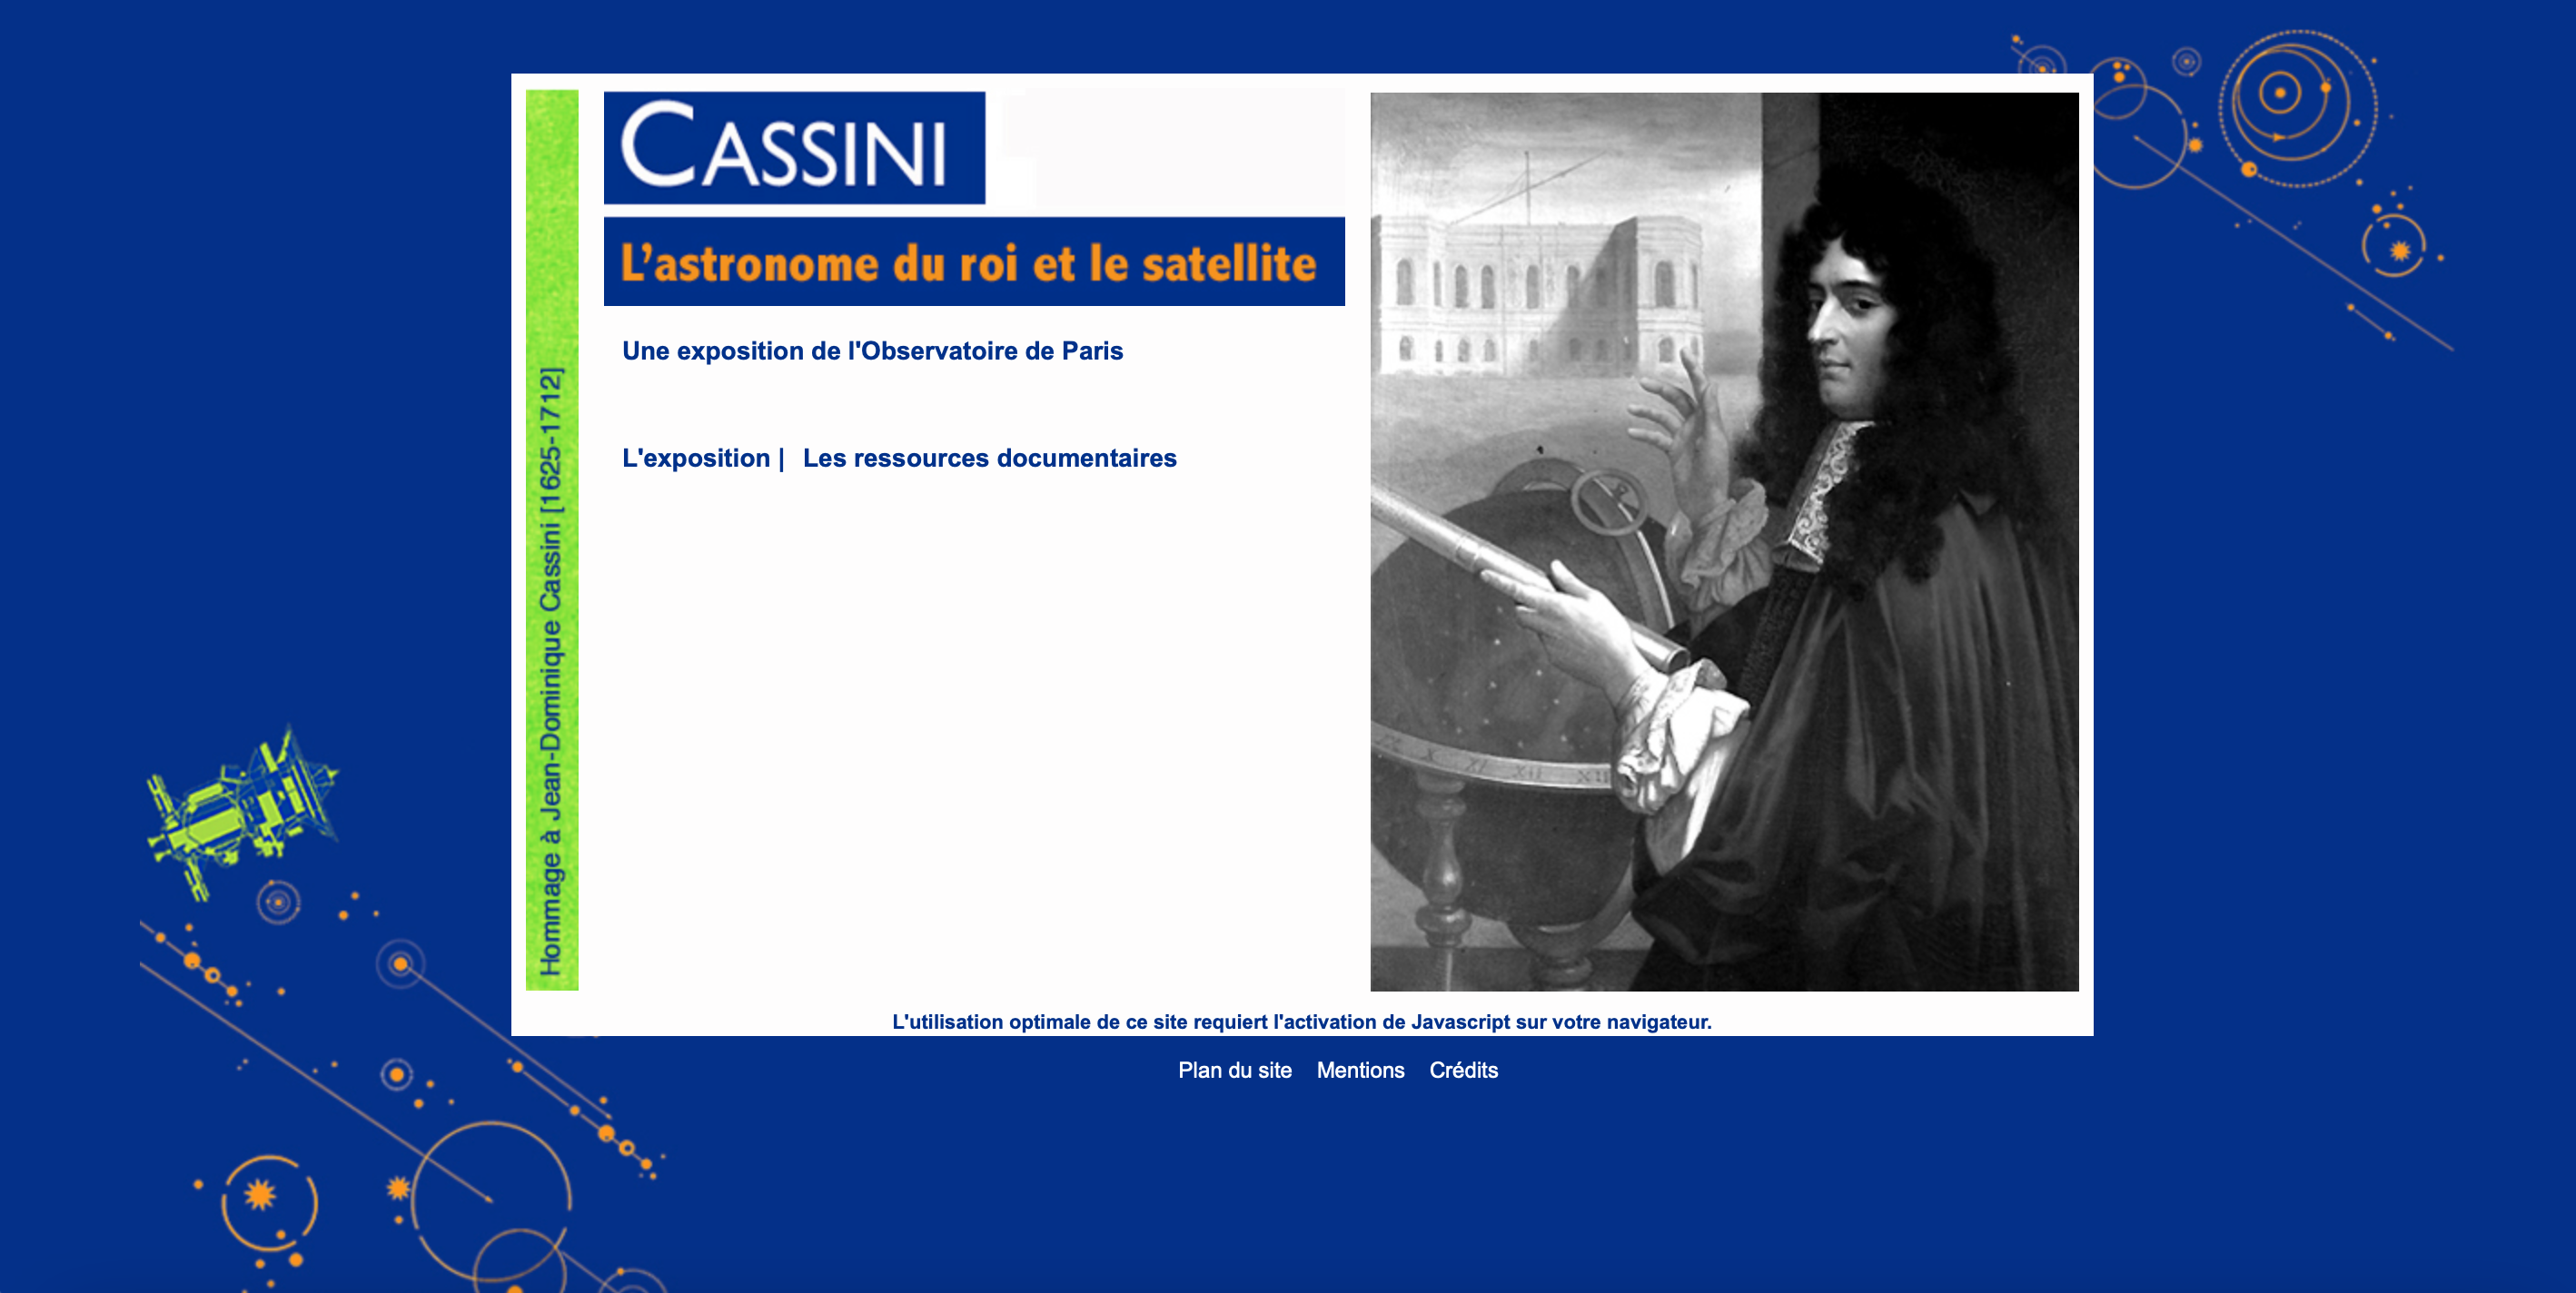
\includegraphics[scale=0.3, angle=0]{images/partie1/expositions/expo-cassini.png}
    \centering
    \end{figure}
	Cette exposition dont la scénographie a fait l'objet du stage de Loriane Buffet en 2012 a été conçue à l'occasion du tricentenaire de la mort de Jean-Dominique Cassini \footnote{\cite{buffetHommageJeanDominiqueCassino2012}. L'exposition peut quant à elle toujours être visitée \href{http://expositions.obspm.fr/cassini/index.php}{ici}.}. Elle accompagne une exposition montée physiquement dans les locaux du bâtiment Perrault de l'Observatoire de Paris (bibliothèque et salle Cassini). Ainsi, elle correspond à un type d'exposition virtuelle différent mais pouvoir avoir accès à un projet précédent au sein de le même institution est tout de même utile. De plus, il est aussi intéressant de remarquer les changements entre l'interface de cette exposition il y a dix ans et ce qui doit être envisagé pour répondre aux attentes qui sont celles des visiteurs d'aujourd'hui. Cela montre aussi que les expositions, virtuelles ou non, sont des objets de leur temps et le reflet des exigences scénographiques alors en vigueur. Les expositions physiques sont limitées dans le temps et l'espace tandis que les expositions virtuelles ne le sont \textit{a priori} pas. Néanmoins, même si elle perdure, l'exposition peut rapidement ne plus satisfaire et devenir, elle aussi, un objet limité dans le temps. Ainsi, la visite de cette exposition sur Cassini peut inviter à se questionner sur la pérennité de ce type d'objet. 
	
	\subsubsection{\textit{Le monde en sphères} à la \acrlong{bnf}}
	\begin{figure}[h]
	\caption{Page d'accueil du site de l'exposition \textit{Le monde en sphères}}
	\includegraphics[scale=0.3, angle=0]{images/partie1/expositions/expo-monde-en-spheres.png}
    \centering
    \end{figure}
	Cette, magnifique, exposition peut,  tout en restant réaliste, représenter une sorte d'objectif en terme de rendu visuel. Réalisée en 2019, elle vient elle aussi accompagner une exposition \textit{in situ} à la \acrshort{bnf} François-Mitterrand. Outre son aspect visuel, l'exposition de la \acrshort{bnf} a pu être une source d'inspiration pour la richesse des pages annexes au contenu principal et notamment la page \textit{Repères}. Ce glossaire est une addition très utile pour aider les visiteurs dans leur navigation en expliquant en quelques mots des notions parfois difficiles et méconnues. De façon analogue, une page \textit{Portraits de savants} est également présente et propose aux visiteurs de courtes biographies de certaines figures majeures pour l'histoire des sciences. Ces guides sont indispensables pour permettre aux visiteurs d'avoir tous les codes en main pour saisir au mieux ce que les auteurs ont cherché à montrer.

	Du fait de sa thématique, elle est proche de l'exposition du projet \acrshort{alfa}. Si la période couverte est plus longue et les objets exposés plus variés, des points de rencontre existent notamment dans la troisième partie intitulée \textit{La sphère dans l'Occident médiéval}. Cela montre que les expositions ne sont pas isolées et qu'elles doivent être replacées dans un contexte global de valorisation de documents manuscrits et de vulgarisation de contenu scientifique. Sur la page d'accueil du site, certains documents à voir absolument sont proposés au sein d'un parcours \textit{En bref} : ce sont les images qui frappent le plus le visiteur, les textes sont là en soutien, pour guider si besoin mais ils ne sont pas le cœur du sujet. La mise en valeur des documents se manifeste aussi par l'existence d'une banque d'images sur le site qui recense l'ensemble des images exposées et permet au visiteur qui le souhaite d'en apprendre plus sur un des documents par un simple clic. À partir de là, le visiteur a également la possibilité de consulter l'image, et le manuscrit dont elle est issue le cas échéant, sur Gallica. C'est ce type de contenu qui est aussi attendu pour l'exposition \textit{Medival skies under(book)cover}.
	
	\subsubsection{\textit{The art of reasoning in medieval mansucripts} à l'Académie royale néerlandaise des arts et des sciences}
	\begin{figure}[h]
	\caption{Page d'accueil du site de l'exposition \textit{Cassini, l'astronome du roi et le satellite}}
	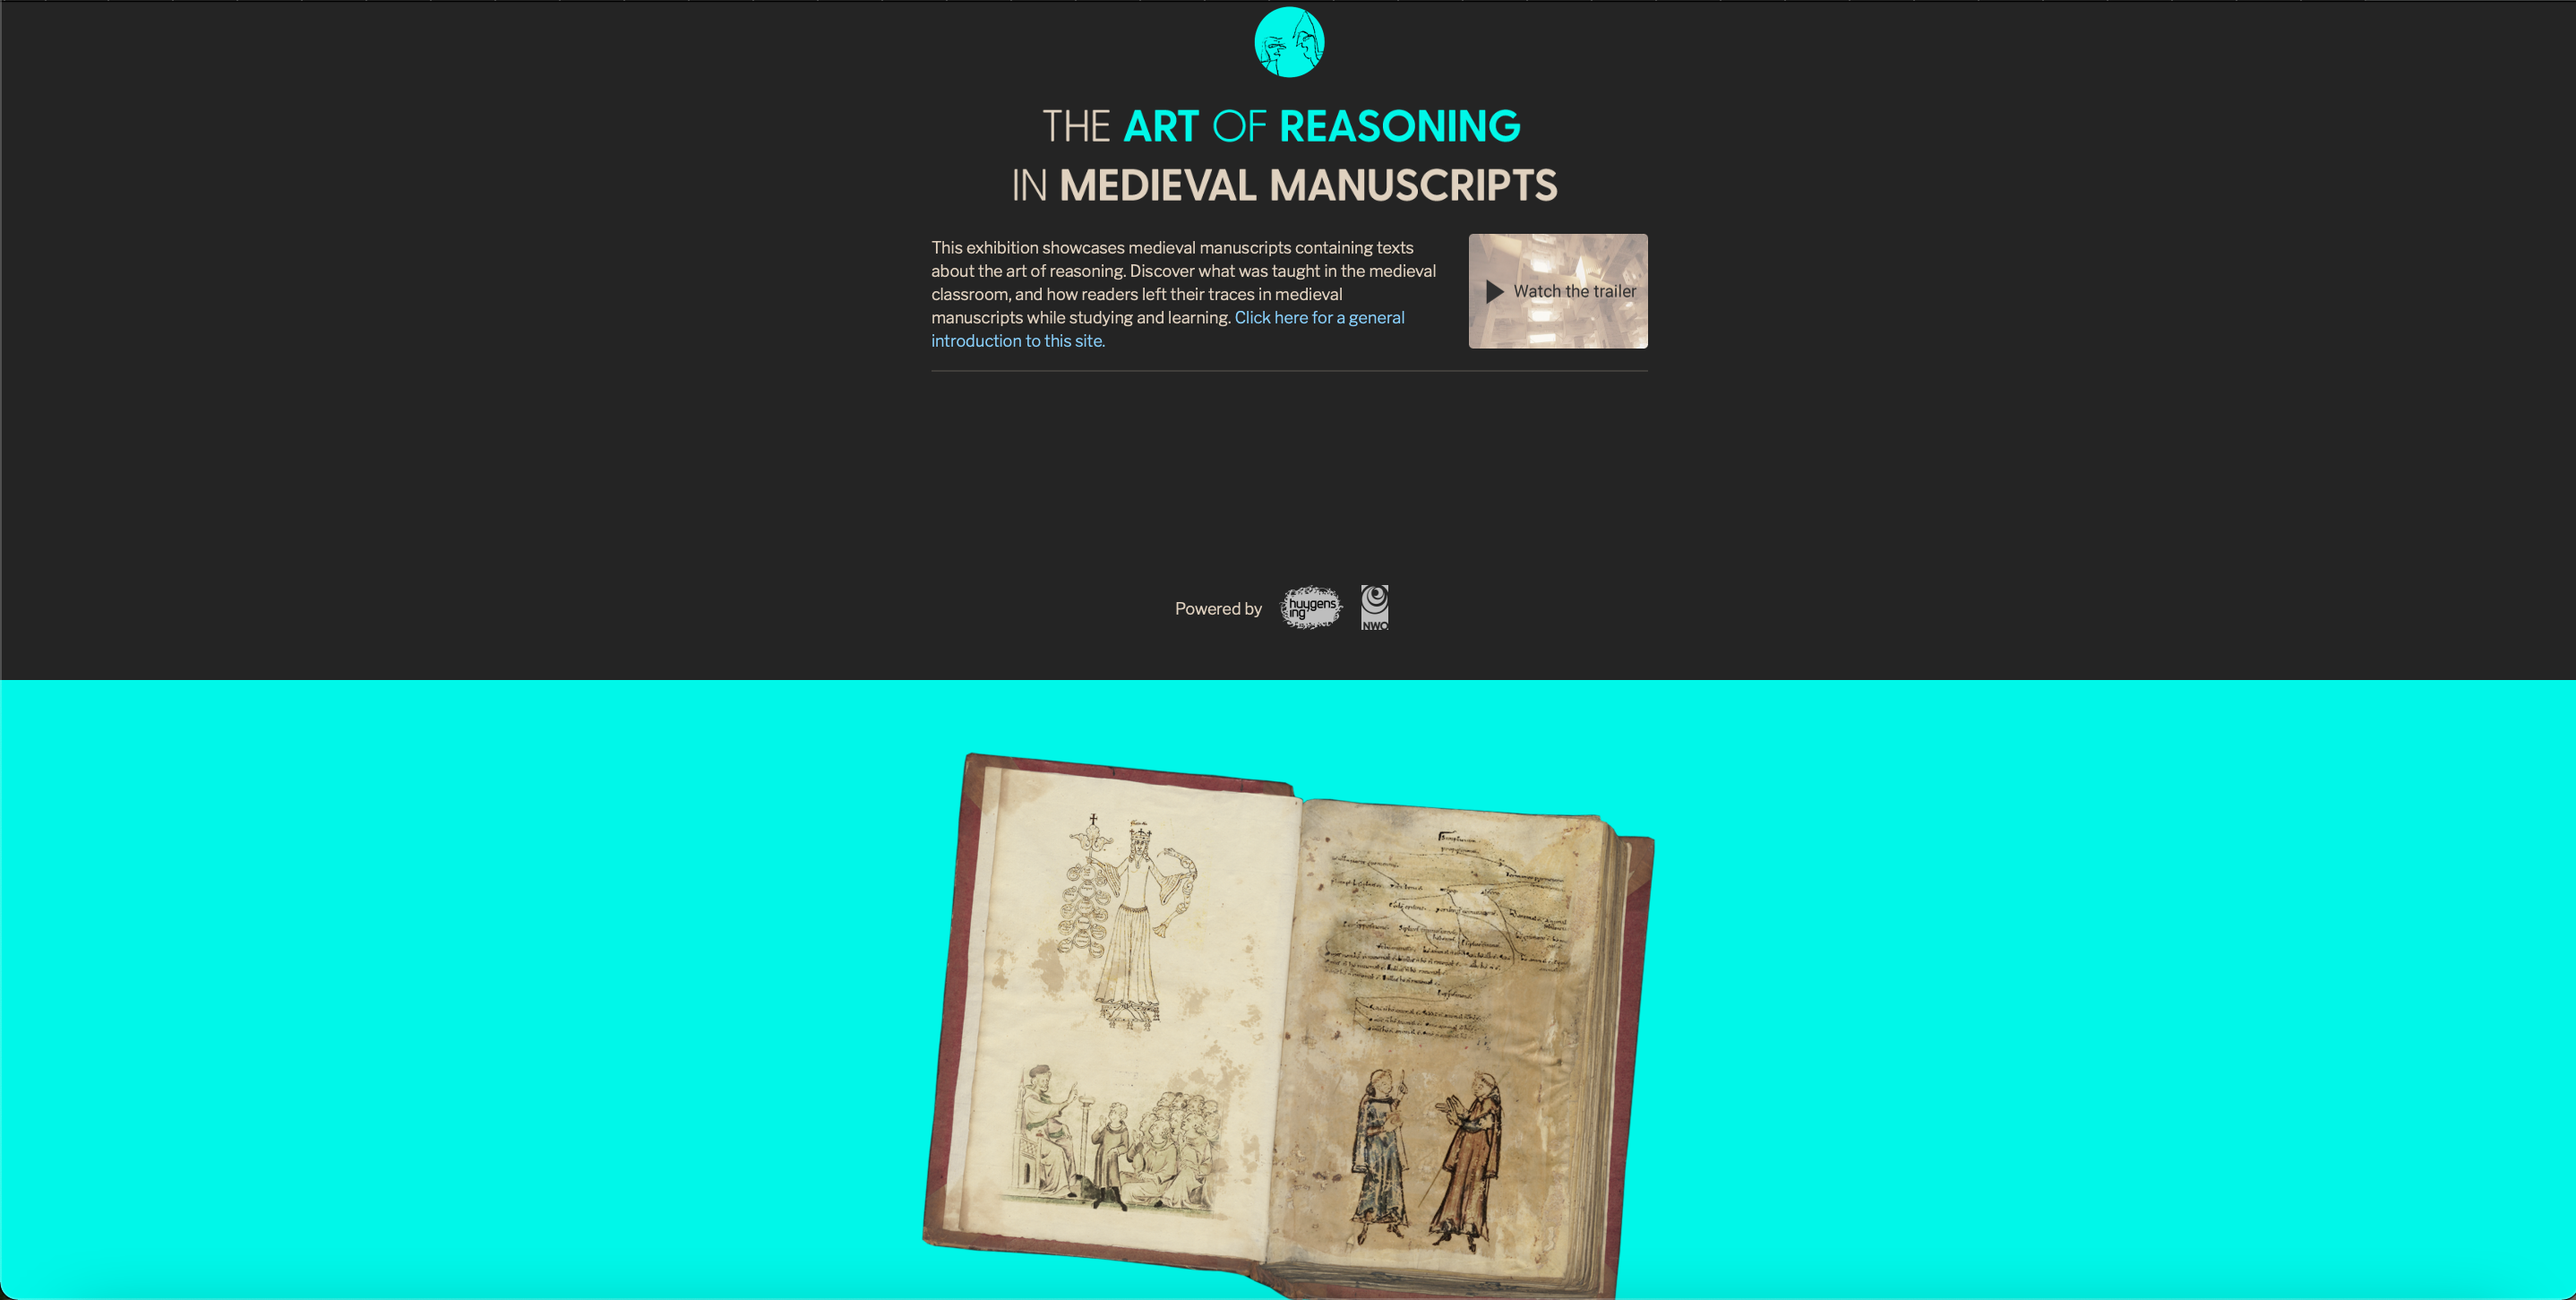
\includegraphics[scale=0.3, angle=0]{images/partie1/expositions/expo-art-of-reasoning.png}
    \centering
    \end{figure}
    Dernière exposition présentée ici, \textit{The art of reasonin in medieval mansucripts} est une exposition néerlandaise conçue dans le cadre du projet de recherche \textit{The Art of Reasoning: Techniques of Scientific Argumentation in the Medieval Latin West (400-1400)} financé de 2016 à 2020 par le Conseil néerlandais de la recherche. Le contexte de réalisation est donc très similaire à celui de l'exposition liée à ce stage. Le site est simple mais plutôt efficace avec quelques efforts pour rendre la navigation un peu interactive. Ainsi, le manuscrit de la page d'accueil est divisé en quatre parties cliquables qui donnent chacune accès à l'un des parcours de navigation du site. Un accès à chacun des manuscrits présentés est également possible via une page dédiée. Pour chaque manuscrit, le lecteur peut ensuite trouver des informations plus précises. C'est de cette exposition que vient l'idée d'une page d'accueil interactive pour l'exposition \acrshort{alfa}. Cela permet d'engager le visiteur et de lui faire prendre en main sa navigation dès son arrivée sur le site. 
    
    À travers les exemples de ces trois expositions, on peut avoir une idée de certains des enjeux liés à ce type de publication allant des simples considérations visuelles à des questions liées à la pérennité. \\
    
    Cette première partie a permis de poser les bases de ce mémoire en évoquant les éléments qui ont également été la base de mon stage. En effet, il était indispensable de cadrer le sujet en présentant le projet \acrshort{alfa} et les documents choisis par l'équipe pour figurer dans l'exposition et en définissant ce qu'est une exposition virtuelle. Une fois cela fait, il est désormais possible de poursuivre en s'intéressant plus concrètement à la scénographie de l'exposition \textit{Medival skies under(book)cover}.